\documentclass[a4paper]{article}
\usepackage{macros-ohp}
\definecolor{vrscolor}{RGB}{255, 255, 255}



%Please make sure the tex is compiled twice to have all the background images displayed correctly.

\title{\Huge \textbf{ \textcolor{vrscolor} {\textless RELATÓRIO DE GESTÃO 2019 \textgreater}}}


\author{\Huge  \textbf{ \textcolor{vrscolor} {\textless Coordenadoria de Planejamento\textgreater\\
	\Huge  \textbf{ \textcolor{vrscolor} {\textless Gerência de Estatística \textgreater \\
	\Huge \textbf{ \textcolor{vrscolor} {\textless Mário Diego Valente \textgreater\\ }}}}}}}
\date{}

\linespread{1.5}




\begin{document}

\begin{titlingpage}
\tikz[remember picture,overlay] \node[opacity=1,inner sep=0pt] at (current page.center){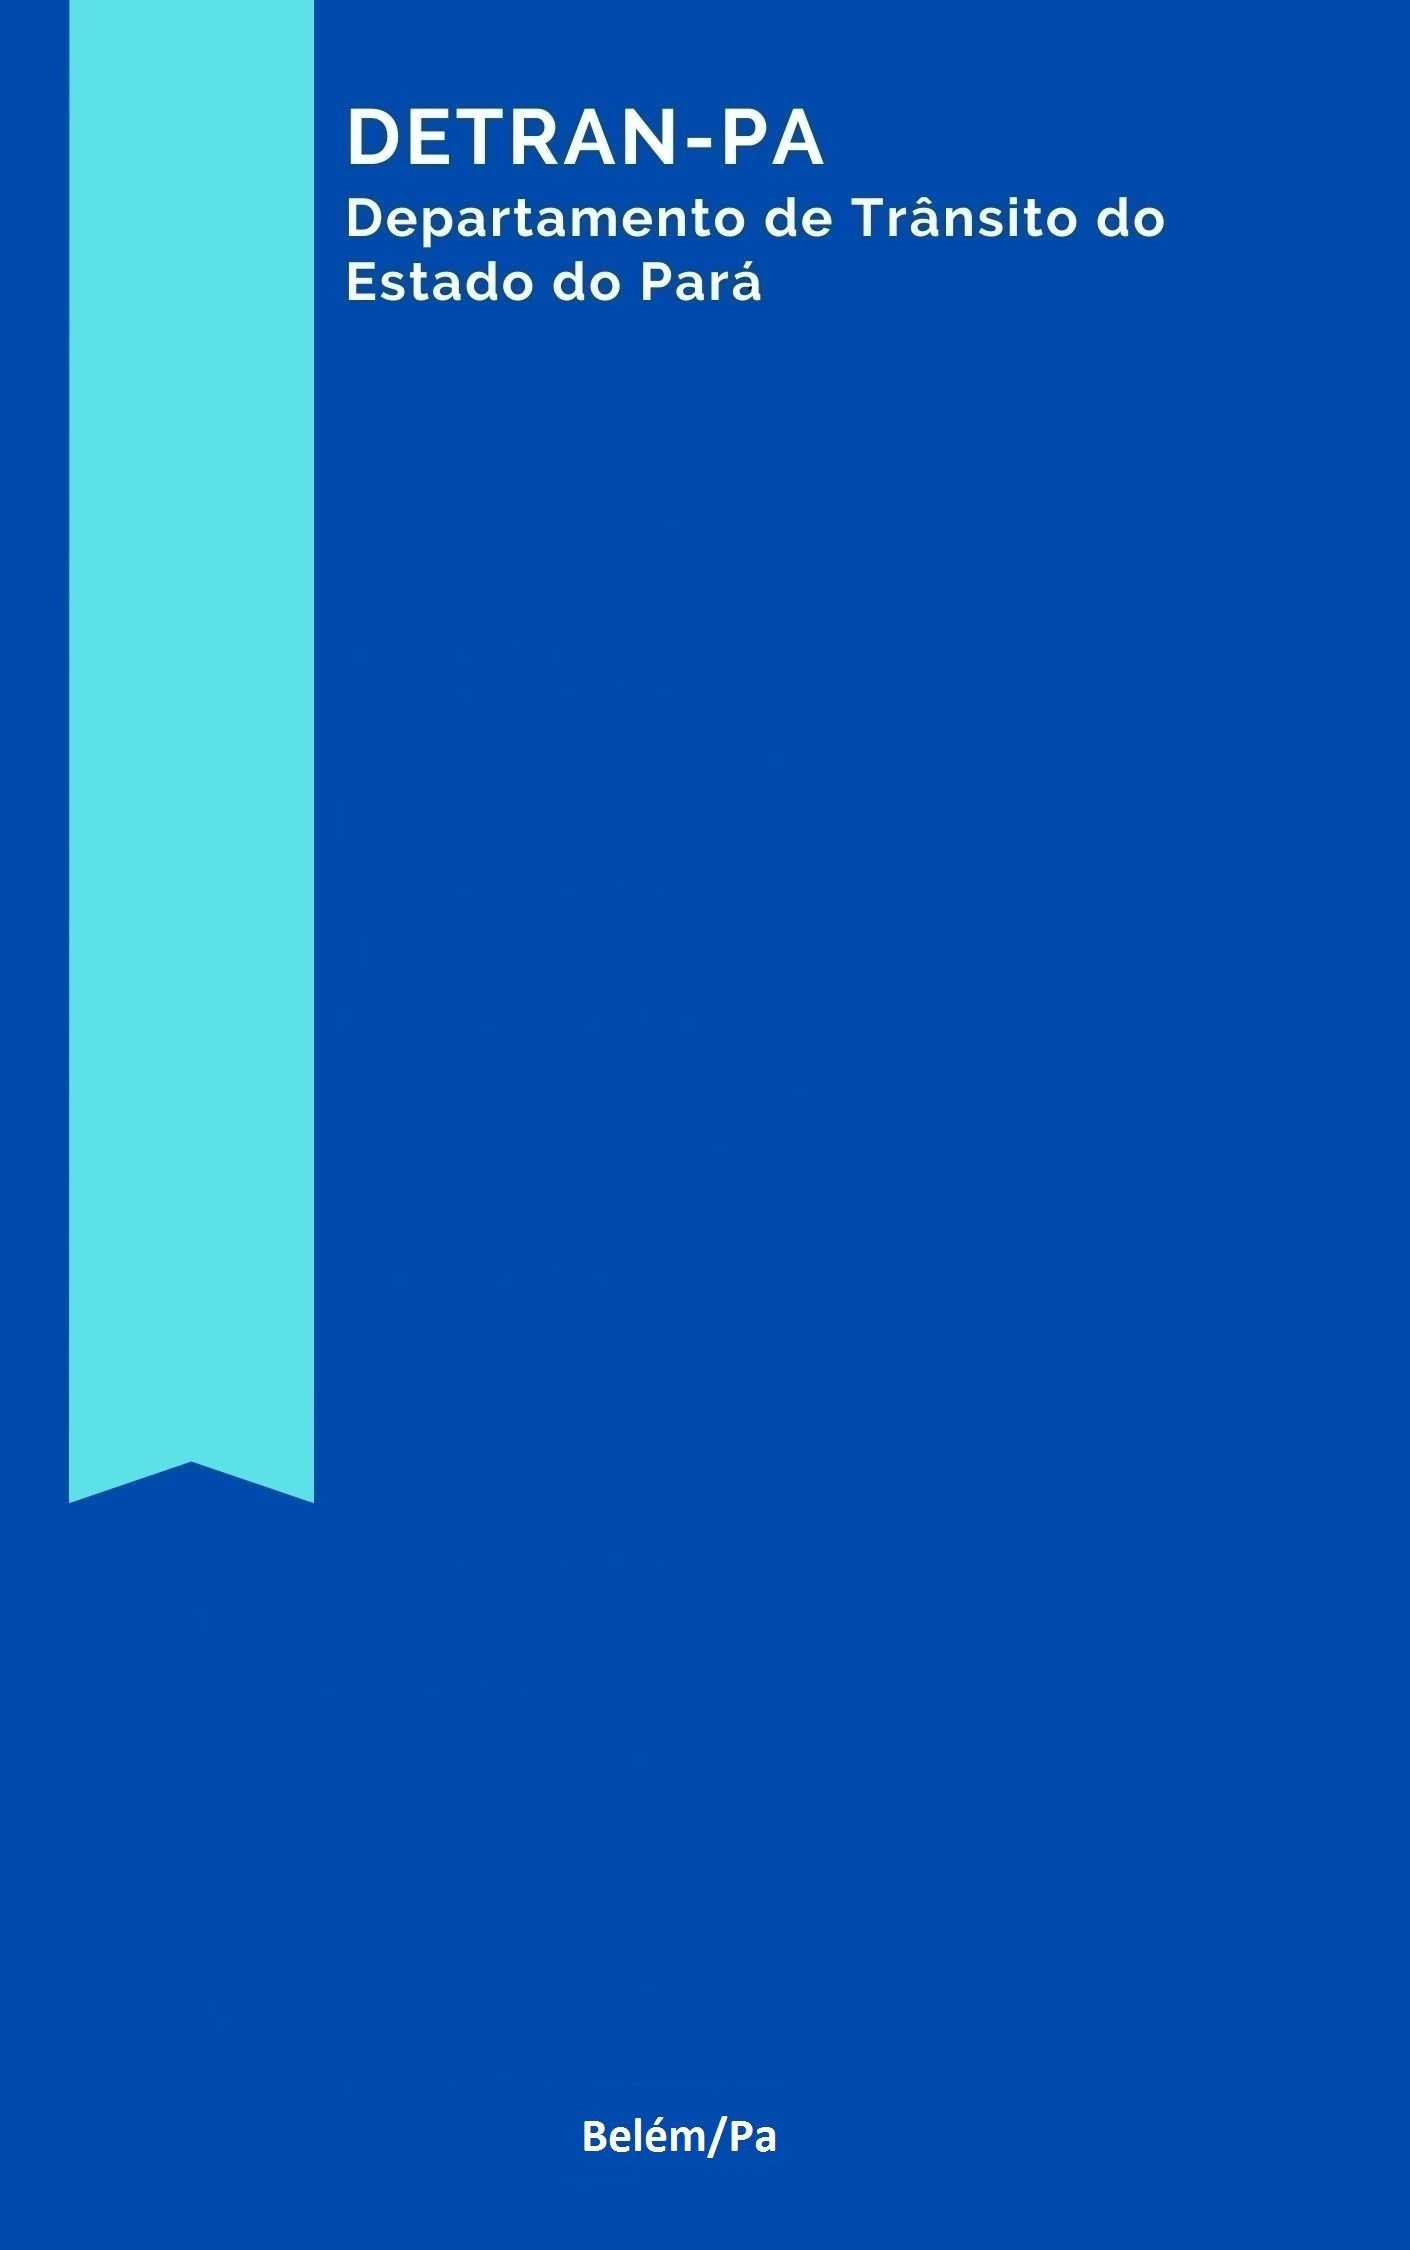
\includegraphics[width=\paperwidth,height=\paperheight]{VRS22-23-report-template-tex/imgs/capa.png}};
\vspace*{3.5cm}
{\let\newpage\relax\maketitle}
\vspace*{\fill}
\end{titlingpage}


\tableofcontents


\newpage

\begin{abstract}
 Em consonância com a Lei n.º 9.503, de 23 de setembro de 1997, que instituiu o 
Código de Trânsito Brasileiro – CTB, bem como com a Resolução n° 514 de 18 de dezembro 
de 2014, que dispõe sobre a Política Nacional de Trânsito, o DETRAN-PA cumpre sua missão 
institucional planejando e destacando orçamento para a execução das ações necessárias ao 
fiel cumprimento dessa determinação legal. Para tanto, elaborou o Plano Plurianual – PPA 
para o quadriênio 2020 a 2023, criando ações para o controle da fiscalização, promoção da 
educação de trânsito, elaboração e execução de projetos de engenharia de trânsito, bem 
como atividades administrativas para a prestação de serviços que garantam a execução da 
política de trânsito no Estado do Pará para o bem estar da sociedade.  
\end{abstract}

\newpage



\newpage
\section{APRESENTAÇÃO}

Apresenta-se Relatório de Monitoramento da Execução das Ações de Educação para o Trânsito, constantes do Plano Plurianual do Departamento de Trânsito do Estado do Pará, referente ao acumulado até segundo quadrimestre de 2019 (janeiro a dezembro), informando o andamento das ações, com objetivo de avaliação da necessidade de interferência da gestão, primando pelo pleno cumprimento dos objetivos programados.\vskip0.3cm

Nas tabelas foram consideradas a previsão orçamentária atualizada para análise da execução orçamentária e financeira, com base no Orçamento Geral do Estado definido no Plano Plurianual.\vskip0.3cm

Para a elaboração desse trabalho e melhor visualização dos resultados, a equipe extraiu dados do sistema SIGPLAN – SEPLAN/PA e Relatórios Mensais Gerenciais (janeiro a dezembro de 2019), podendo sofrer alterações futuras conforme inserção de novos dados no sistema.\vskip0.3cm



\newpage
\section{Aspectos Gerais}

Criado em dezembro de 1972 pela Lei n.º 4.444, o Departamento de Trânsito do Estado do Pará- DETRAN/PA surgiu em forma de autarquia com autonomia técnica administrativa, financeira e patrimonial, visando cuidar do Trânsito no Estado do Pará. O Departamento de Trânsito do Estado do Pará é órgão executivo integrado ao Sistema Nacional de Trânsito e ao Sistema de Segurança Pública do Estado, além de vinculado à Secretaria Executiva de Segurança Pública e Defesa Social do Pará.\vskip0.3cm

O Sistema Nacional de Trânsito - SNT é composto pelos órgãos normativos, consultivos, executivos e rodoviários nas diferentes esferas de governo, tal organização pode ser visualizada na figura 1.\vskip0.3cm


\section{Organização Administrativa}


A reorganização do órgão foi definida pela Lei n° 7.594, de 28 de dezembro de 2011, que começou a vigorar a partir da publicação ocorrida em 29 de dezembro do mesmo ano, da qual ainda não foi concluído o novo Regimento Interno.\vskip0.3cm

Art. 2°. São funções básicas do Departamento do Estado do Pará:\vskip0.3cm

\begin{enumerate}

\item Cumprir e fazer cumprir a legislação e as normas de trânsito, no âmbito de suas atribuições;
\item Realizar, fiscalizar e controlar o processo de formação e reciclagem de condutores, expedir permissão para dirigir, expedir e cassar licença de aprendizagem, autorização para conduzir ciclomotores e Carteira Nacional de Habilitação;
\item Vistoriar, registrar, emplacar, selar a placa, e licenciar veículos, expedindo Certificado de Registro de Veículos – CRV e Certificado de Registro e Licenciamento de Veículos – CRLV;
\item Estabelecer, em conjunto com a Polícia Militar, as diretrizes para o policiamento ostensivo de trânsito;
\item Executar a fiscalização de trânsito, autuar e aplicar as penalidades por infrações e medidas administrativas cabíveis previstas nos artigos 21 e 22 do CTB nas áreas urbana e rural;
\item Supervisionar o controle de aprendizagem para conduzir veículos automotores;
\item Fiscalizar o nível de emissão de poluentes e ruídos produzidos pelos veículos automotores ou pela sua carga, além de dar apoio às ações específicas dos órgãos ambientais locais quando solicitado;
\item Coletar dados estatísticos e elaborar estudos sobre acidentes de trânsito e suas causas;
\item Arrecadar valores provenientes de estada e remoção de veículos e objetos;
\item Articular-se com os demais órgãos do Sistema Nacional de Trânsito no Estado, sob coordenação do respectivo CETRAN;
\item Emitir Autorização Especial de Trânsito – AET;
Parágrafo único. No exercício de sua missão, o Departamento de Trânsito do Estado do Pará – DETRAN/PA poderá celebrar convênios com órgãos executivos de trânsito nos municípios integrados ao Sistema Nacional de Trânsito no Estado do Pará, com vistas ao fornecimento de dados cadastrais dos veículos registrados e dos condutores habilitados, para fins de imposição e notificação de penalidades e de arrecadação de multas nas áreas de suas competências.
\end{enumerate}





\section{Competencias Administrativa}

O Departamento de Trânsito do Estado do pará possui varias diretorias, uma delas e a Diretoria Técnica e Operacional (DTO), que se divide em um tripé muito importante:

\begin{itemize}
    \item Educação;
    \item Engenharia;
    \item Fiscalização
\end{itemize}


A missão da coordenadoria de Educação de Trânsito é desenvolver ações que despertem tanto nos condutores quando nos pedestres atitudes mais seguras no trânsito. Estas ações assumem o formato de campanhas educativas, palestras informativas e cursos de capacitação para os interessados em contribuir com um trânsito seguro e cidadão.\vskip0.3cm

Para que este trabalho seja desenvolvido de forma mais eficaz em todo o Estado do Pará em seus 144 municípios, a Coordenadoria de Educação dividi-se em 4 gerências e suas respectivas especialidades.\vskip0.3cm 


\subsection{Gerência de Cultuta de Trânsito}
À gerência de cultura de trânsito, diretamente subordinada à Coordenadoria de Educação do DETRAN-PA, compete:
\vskip0.3cm



\begin{itemize}
\item Planejar, elaborar e executar o desenvolvimento de ações intersetoriais educativas de trânsito realizadas junto às instituições públicas privadas, organizações internacionais, não governamentais, entidades e empresas;
\item Elaborar e executar programas e projetos relacionados a promoção de um nova cultura de trânsito que valorize a qualidade de vida, a promoção da paz e respeito ao  meio ambiente;
\item Fomentar percerias com a sociedade civil organizada a fim de disseminar hábitos e comportamentos seguros no trânsito para a redução dos riscos de acidnetes;
\item Integrar-se às instituições educacionais públicas e privadas de ensino básico e superior, através de ações interdisciplinares, para a promoção de novos valores sociais a partir do tema trânsito;
\item Mobilizar voluntários sociais para a atuação em campanhas de prevenção de acidentes e segurança no trânsito com a valorização da cidadania ativa;
\item Participar de eventos, feiras e espaçoas culturais disseminando a cultura  de segurança no trânsito;
\item Desenvolver metodologias de trabalho específicas para realizar ações culturais relacionadas ao comportamento seguro no trânsito;
\item Articular-se às ações das políticas públicas que estejam relacionados à educação  e promoção da ética e da cidadania;
\item Apresentar proposta ao setor de comunicação a divulgação na mídia e nos diversos meios de comunicação de informações sobre projetos e ações desenvolvidas sobre a culura de trânsito seguro e responsável;
\item Promover parcerias com instituições de ensino superior para realizar pesquisas sociológicas, antropológicas, jurídicas e outras correlatas a area de tânsito enquanto fenômeno social;
\end{itemize}




\subsection{Gerência de Integração Educacional}
À gerência de integração Educacional, diretamente subordinada à Coordenadoria de Educação do DETRAN-PA, compete:
\vskip0.3cm 

\begin{itemize}
\item Planejar, realizar e monitorar trabalho de percusão visando a promoção de parcerias com os órgãos e entidades que estejam relacionados com os programas, projetos e ações educativas da CED;
\item Orientar e acompanhar o desenvolvimento de ações relizadas pelas instituições governamentais e não governamentais parceiras do Programa de Educação do DETRAN-PA;
\item Propor e fomentar parcerias que visem à implementação, a manutenção e ao aperfeiçoamento de ações ligadas às diversas políticas, com vistas a garantir a visão holística das ações da CED;
\item Fomentar, junto aso parceiros, a capacitação e formação de agentes multiplicadores em arte-educação;
\item Integrar-se aos projetos de educação e segurança nas escolas, desenvolvidas pelo Sistema Estadual de Segurança Pública e Sistema Ensino Público e Privado;
\item Integrar-se aos projetos e programas desenvolvidos na esfera federal, estadual, municipal, nas empresas e ONG’S promovendo ações educativas de trânsito seguro;
\item Disseminar entre os setores do DETRAN-PA a prticipação dos servidores em campanhas educativas internas e nas atividades promovidas pelo òrgão;
\item Subsidiar as CED com informações específicas das atividades pertinentes a sua area de atuação;
\item Propor a CED o aperfeiçoamento dos procedimentos internos, visando a melhoria contínua dos trabalhos desenvolvidos;
\end{itemize}


\subsection{Gerência de Programas e Projetos Pedagógicos}

À gerência de Programas e Projetos Pedagógicos, diretamente subordinada à Coordenadoria de Educação do DETRAN-PA, compete:
\vskip0.3cm 

\begin{enumerate}
\item Planejar e elaborar projetos pedagógicos para dar suporte às ações das demais gerências da CED;
\item Articular-se em rede aos programas e projetos desenvolvidos por outros órgãos do Governo do Estado como forma de ampliar intersetorialmente as ações de Educação de Trânsito;
\item Avaliar e supervisionar os programas, projetos e ações pedagógicas da Educação de Trânsito;
\item Desenvolver metodologias específicas para os programas  e projetos pedagógicos;
\item Fornecer subsídios para o planejamento das ações a serem desenvolvidas pela CED;
\item Participar das operações programadas pelo DETRA-PA, em parceria com a engenharia, fiscalização e outros setores afins;
\item Orientar, acompanhar e supervisionar o desenvolvimento de ações relizadas pelas instituições governamentais e não governamentais parceiras da CED;
\item Subsidiar a CED com informações específicas das atividades pertinentes à sua área de atuação;
\item Propor a CED o aperfeiçoamento das ações, visando à melhoria e a qualidade do atendimento às demandas;
\end{enumerate}



\subsection{Gerência de Escola Pública de Trânsito}

À gerência de Escola Pública de Trânsito, diretamente subordinada à Coordenadoria de Educação do DETRAN-PA, compete:

\begin{enumerate}
\item Planejar, elaborar, executar e acompanhar o desenvolvimento de projetos, cursos e ações educativas de trânsito voltados ao exercício da cidadania;
\item Planejar e executar cursos de capacitação para agentes multiplicadores em educação de Trânsito de acordo com os programas e projetos desenvolvidos no DETRAN-PA;
\item Propor a realização de parcerias com outros órgãos e instituições governamentais para realizar cursos de reciclagem de condutores e de aperfeiçoamento para as categorias do trânsito;
\item Planejar, executar e monitorar curso teórico de 1ª habilitação para alunos do ensino médio de acordo com as diretrizes da Política Nacional de Trânsito (PNT) e Resoluções do CONTRAN;
\item Planejar, executar e acompanhar cursos de formação especializada para categorias profissionais do trânsito e outros cursos de acordo com Resolução do CONTRAN e Legislação vigente;
\item Propor o desenvolvimento de metodologias para a formação continuada da equipe da CED;
\item Elaborar o projeto pedagógico de acordo com a Lei de Diretrizes e Bases da Educação Nacional (LDB), dos Parâmetros Curriculares Nacional (PCN), das Diretrizes do DENATRAN e os objetivos e diretrizes da Política Nacional de Trânsito;
\item Articular-se às instituições educacionais públicas e privadas de ensino superior, a fim de desenvolver estudos, pesquisas e produzir conhecimentos interdisciplinares sobre a temática trânsito;
\item Promover a avaliação das ações de educação de trânsito através da coleta de dados e realização de pesquisas.
\end{enumerate}



\section{Missão, Visão, Valores}

Em observância ao que dispõe o Código de Trânsito Brasileiro, Resoluções do Conselho Nacional de Trânsito, Portarias e Deliberações do Conselho Nacional de Trânsito, bem como Portarias do Departamento Nacional de Trânsito e as diretrizes da Política Nacional de Trânsito, o Departamento de Trânsito do Estado do Pará possui as seguintes diretrizes de gestão.


\subsection{Missão Institucional}

Assegurar a execução da Política Nacional de Trânsito no Estado do Pará, de forma articulada e integrada com os demais agentes sociais, zelando pelo cumprimento da lei, com vistas à preservação e valorização da vida e do bem estar da sociedade.


\subsection{Visão Institucional}

Ser um órgão de trânsito reconhecido por ações voltadas à universalização dos serviços, valorização da vida, promoção da cidadania, equidade e civilidade no trânsito do Estado do Pará, com credibilidade, em um cenário integrado de trânsito seguro e sustentável para a sociedade.

\subsection{Valores Institucional}

\begin{itemize}
    \item Respeito à Vida; 
    \item Segurança no Trânsito;
    \item Eficiência e Ètica nos Serviços;
    \item Valorização dos Serviços;
    \item Universalização do Acesso aos Serviços;
\end{itemize}


\subsection{Matriz SWOT}

As matrizes, além de viabilizar e agilizar as análises, têm uma importante função que é quantificar as análises de ações e/ou atividades que normalmente são qualificativas e, portanto, passíveis de questionamento nas reuniões para aprovação do PPA. As matrizes mais utilizadas e que você precisa saber são: SWOT, BCG, Análise de Forças Competitivas; Avaliação de Entrantes Potenciais, CVA, Matriz de Ansoff e Poítica Direcional. Sendo que, a adotada pelo presente estudo será a matriz swot.\vskip0.3cm
 
Considerando a matriz SWOT (Strengths, Weaknesses, Opportunities and Threats), ou simplesmente FOFA (Forças, Frquezas, Oportunidades e Ameaças). A matriz SWOT é sempre feita em quadrantes, ou seja, em quatro quadrados exatamente iguais, sendo um demostrativo qualitativo de aspectos positivos e negativos de seu produto e/ou ação. \vskip0.3cm

Construindo  os quadrantes, temos:
\vskip0.3cm


\begin{itemize}
\item FORÇAS:  aqui você vai listar  em tópicos os aspectos mais positivos da organização em relação ao seu produto, serviço ou unidade de negócio. São variáveis com boa possibilidade de controle pela sua empresa e são fatores de elevada importância para seu PPA;
\item FRAQUEZA: aqui você vai listar em tópicos os aspectos mais negativos da empresa com relação ao seu produto, serviço ou unidade de negócio. São variáveis com boa possibilidade de controle pela sua empresa e são fatores de elevada importância para o seu PPA;
\item OPORTUNIDADES: aqui você vai listar em tópicos os aspectos mais positivos em relação ao mercado, para seu produto, serviço ou unidade de negócio. São variáveis normalmente incontroláveis pela sua empresa e são fatores de elevada importância para o seu PPA;
\item AMEAÇAS: aqui você vai listar em tópicos os aspectos externos mais significativos para insegurança quanto ao sucesso do seu produto, serviço ou unidade de negócio. São variáveis normalmente incontroláveis pela sua empresa e são fatores de elevada importância para o seu PPA.
\end{itemize}

Foi realizada revisão pela equipe técnica participante do processo de elaboração do planejamento dos cenários com base no cenário do ano anterior, resultando no seguinte diagnóstico simplificado do DETRAN-PA, demostrado nos quadros abaixo.
\vskip0.3cm

A matriz swot resulta numa análise muito prática dos aspectos que serão comtemplados estratégicamente no seu PPA, tais como vantagens a serem utilizadas, aspectos que requerem ações para aperfeiçoamento e adequação pelos riscos que representam.
\vskip0.3cm

\section{Avaliação dos Programas e Ações}
\subsection{Programa Segurança Pública}

Com o objetivo de prevenir acidentes de trânsito no Estado do Pará, o Departamento Trânsito compõe, com os demais órgãos de segurança pública, o Programa “Segurança Pública”, no qual participa de 12 ações¹ para viabilizar sua atuação na prestação de serviços de habilitação de condutores, registro de veículos, educação e fiscalização de trânsito, engenharia de trânsito, além da promoção da infraestrutura física para garantir atendimento de qualidade à população usuária.

\subsection{Setor de Educação}

Em 2019 a ação de educação o DETRAN viabilizou a realização de 493 ações educativas, cumprindo 108\% da meta física prevista, conforme se observa na tabela 2. 

Para viabilizar essas ações, foram gastos recursos no valor total de R\$ (1.024.293,18), correspondentes a apenas 16\% da dotação orçamentária prevista inicialmente, conforme se verifica na Tabela 2.


\subsection{Projetos Gerenciais}

No que tange a execução das ações educativas realizadas pelas 4 gerências que compõem a Coordenadoria de Educação, far-se-á uma descrição discriminadas nas atividades desempenhas por cada uma no período de janeiro a dezembro de 2019, conforme tabelas a seguir. 


\subsubsection{Atividades: Gerência de Cultuta de Trânsito}

De acordo com a tabela 4 pode-se observar 12 tipos de atividades diferentes realizadas pela Gerência de Cultura de Trânsito, desenvolvendo diversos projetos vinculados ao Planejamento Pluri Anual de 2016 a 2019. Nesse contexto, a Gerência de Cultura de Trânsito desenvolveu diversos Projetos dos quais os resultados constam na tabela 4.\vskip0.3cm


O Projeto DETRAN nas Empresas, cujo objetivo foi realizar palestras sobre a temática trânsito para colaboradores de diversas Empresas Públicas e Privadas, refletindo sobre a segurança no trânsito e assimilar medidas preventivas, que os façam adotar práticas seguras durante a jornada de trabalho e no seu trajeto do dia a dia.\vskip0.3cm


A partir das estratégias, as ações metodológicas serão baseadas na realização de palestras interativas com os participantes, resguardando sempre suas experiências profissionais e distribuição de material educativo, como folders, catálogos e brindes, como forma de reforço do conteúdo ministrado, incentivando-os para ações futuras e abordando os temas: Ètica e Cidadania de Trânsito, Comportamento Seguro no Trânsito, Direção Defensiva, Fatores de Risco no Trânsito, Álcool e Direção e Noções de Legislação de Trânsito.
\vskip0.3cm
  
No período de abril a dezembro foram realizadas 19 palestras em várias empresas com um público de 1.824 pessoas atendidas. Dentre as empresas atendidas, destacam-se, Agropalma, Celpa, Hileia, Natura, Empresas de Ônibus, Mônaco, Pará-Segurança, etc. 
\vskip0.3cm

O Projeto Reeducando com Valor/Cumpridores de Medidas Alternativas, cujo objetivo foi realizar palestras sobre a temática trânsito para pessoas que foram condenados ao cumprimento de prestação de serviços gratuito à comunidade, beneficiado com a suspensão condicional do processo, por transação penal ou sentença condenatória, mediante aplicação de penas e medianas alternativas, aplicadas pelos Juizados Penais e Juizados Especiais Criminais da Região Metropolitana de Belém, com base no Convênio celebrado entre o Tribunal de Justiça do Estado Pará, por meio da Vara de Execução das Penas e Medidas Alternativas (VEPMA) e a Escola Pública de Trânsito do DETRAN-PA. 
\vskip0.3cm

As ações metodológicas serão baseadas na realização de palestras interativas com os reeducando e distribuição de material educativo, como folders, catálogos e brindes, como forma de reforço do conteúdo ministrado, incentivando-os para ações futuras e abordando os temas: Ética e Cidadania de Trânsito, Comportamento Seguro no Trânsito, Álcool e Direção, Noções de Legislação de Trânsito, Fatores de Risco no Trânsito, Normas de Circulação e Conduta e Direção Defensiva. No período de janeiro a dezembro foram realizadas 37 palestras nas dependências da Escola Pública de Trânsito, com um público de 152 pessoas atendidas, que, em sua maioria, sofreram algum acidente de trânsito.
\vskip0.3cm


O Projeto DETRAN nas Comunidades, cujo objetivo foi realizar palestras sobre a temática trânsito criando teias de relações sociais entre os moradores e o poder público, implementando e difundindo os conceitos de segurança no trânsito em vários segmentos da sociedade.
\vskip0.3cm

Desta forma, o projeto estimula a sociedade civil a identificar as problemáticas locais propondo soluções adequadas e específicas a estas comunidades, aproveitando uma estrutura de organização que já existe para inserir os conceitos de educação no trânsito, mesmo após as atividades sazonais do DETRAN.
\vskip0.3cm

Durante o período de janeiro a dezembro foram realizadas 18 palestras nas comunidades, igrejas, associações e escolas, com um público de 385 crianças e 1.455 adultos atendidos, que em torno de 75\% relataram algum familiar já sofrera acidentes e/ou incidentes no trânsito.\vskip0.3cm


O Projeto Transitando no Bares, cujo objetivo é realizar abordagens educativas aos clientes dos bares, de caráter informativo e preventivo e serão pautadas no estabelecimento de um canal de comunicação entre os Agentes de Educação e o público alvo. Esse processo de comunicação e aprendizagem será mediado por relações dialógicas, esquetes, apresentações teatrais e dinâmicas para interação com público, que permitam a estes envolverem-se na situação reconhecendo a responsabilidade pessoal de cada um na mudança do panorama atual. 
\vskip0.3cm

Nesse momento haverá a distribuição material pedagógico e brindes específicos, prática importante para a difusão dos ideais da campanha, pois eles contêm mensagens precisas para reflexão sobre a situação de optar por álcool ou direção. O projeto visa estimular a reflexão sobre o ato de “beber ou dirigir”, assim como promover outros comportamentos como o “amigo da vez”, a “carona legal” ou “se beber vá de táxi”.No período de maio a dezembro foram realizadas 7 imersões em 28 bares, com um público de 2.177 clientes abordados e 232 testes do etilômetro.\vskip0.3cm


\subsubsection{Atividades: Gerência de Integração Educacional}

De acordo com a tabela 5 pode-se observar 09 tipos de atividades diferentes realizadas pela Gerência de Integração de Trânsito, desenvolvendo diversos projetos vinculados ao Planejamento Pruri Anual de 2016 a 2019. Nesse contexto, a Gerência de Integração de Trânsito desenvolveu diversas Ações dos quais os resultados constam na tabela 5.\vskip0.3cm

O Projeto DETRAN nas Escolas, cujo objetivo foi realizar palestras sobre a temática trânsito para alunos e professores das Escolas Públicas e Privadas, refletindo sobre a segurança no trânsito e adotando práticas seguras durante o seu trajeto do dia a dia.\vskip0.3cm

No período de julho a dezembro foram realizadas 51 palestras em Parceria com o Projeto Territórios da Paz (TERPAZ), sendo 07 no Ensino Maternal, 22 no Ensino Fundamental e 11 no Ensino Médio, perfazendo um total de 4.376 crianças assistidas, 1.197 adultos (pais/parentes) e 57 professores.\vskip0.3cm

O Projeto Blitz Educativas, cujo objetivo é fazer uma Parada Educativa Veicular aos condutores de veículos que trafegam nos principais polos de entrada e saída dos municípios estratégicos, durante as grandes operações sazonais. O modus operantis da ação, funciona em três etapas: \vskip0.3cm


\begin{itemize}
\item 1ª abordagem Veicular (sempre) é feita pelo Agente de Trânsito (Municipal/Estadual), Guarda Municipal e Polícia Militar;
\item 2ª abordagem é feita pelo Agente de Educação de Trânsito, informando, esclarecendo e oriantado os condutores sobre os fatores de risco no trânsito;
\item 3ª abordagem é feita um levantamento observacional (planilha) dos fatores de risco, presente ou não em cada veículo.
\end{itemize}

Caso o veículo se encontrasse em situação normal, o conduto e passageiros recebiam informações sobre a campanha desenvolvida pelo DETRAN-PA, onde os educadores informavam sobre os principais fatores de risco no trânsito. Caso o veículo apresentasse alguma situação de risco no trânsito, os agentes de educação entregavam o material de campanha e alertavam os condutores e passageiros da necessidade de seguir os procedimentos corretos no trânsito, de forma a diminuir a possibilidade de acidentes de trânsito.\vskip0.3cm

No período de julho a dezembro foram realizadas 36 Blitz Educativas, abordando 4.642 veículos, onde mais de 85\% dos veículos foram automóveis de passeio. Durantes as ações nas blitz educativas, foram feitos levantamentos observacionais sobre os aspectos de riscos encontrados nos veículos abordados com correção educativa imediata, totalizando 2.176 fatores de risco encontrados, sendo os de maior incidência: passageiro no banco de tras sem cinto de segurança, objetos soltos, crianças sem dispositivos de retenção, animais solto e excesso de passageiros.\vskip0.3cm



\subsubsection{Atividades da Gerência de Programas e Projetos Pedagógicos de Trânsito}

De acordo com a tabela 6 pode-se observar 07 tipos de atividades diferentes realizadas pela Gerência de Programas e Projetos Pedagógicos de Trânsito, desenvolvendo diversos projetos vinculados ao Planejamento Pluri-Anual de 2016 a 2019. Nesse contexto, a Gerência de Programas e Projetos Pedagógicos de Trânsito desenvolveu diversas Ações dos quais os resultados constam na tabela 6.\vskip0.3cm

O Projeto DETRAN nas Faixas de Travessia de Pedestre, cujo objetivo é fazer abordagens educativas com intervenções positivas durante a travessia nas faixas de pedestres em frente aos principais locais de aglomeração e fluxos de pessoas, como Farmácias, Mercados, Comércios, Shopping, etc., com intuito de orientar e auxiliar no atravessar da via de forma correta e com segurança tanto dos pedestres quanto dos ciclistas.
\vskip0.3cm

Durante o período de julho a dezembro foram realizadas 7 intervenções nas Faixas de Travessia de Pedestres com 1.650 pessoas orientadas. 

\subsubsection{Atividades da Gerência de Escola Pública de Trânsito}

De acordo com a tabela 7 pode-se observar 11 tipos de atividades diferentes realizadas pela Gerência de Programas e Projetos Pedagógicos de Trânsito, desenvolvendo diversos projetos vinculados ao Planejamento Pluri Anual de 2016 a 2019. Nesse contexto, a Gerência de Escola Pública de Trânsito desenvolveu diversas Ações dos quais os resultados constam na tabela 7.\vskip0.3cm

O Projeto Curso de Mototaxistas, cujo objetivo é fazer a formação de profissionais com curso Especializado Obrigatório de Mototaxistas e Motofretista para os profissionais liberais. O Curso foi instituído pela Resolução do CONTRAN Nº410 de 2012, e tem por objetivo garantir aos motociclistas profissionais a aquisição de conhecimentos, a padronização de ações e atitudes de segurança no trânsito.\vskip0.3cm

Durante o período de agosto a dezembro foram realizados 15 turmas com supervisão da equipe pedagógica, totalizando 353 alunos formados.
































\end{document}